\documentclass[11pt]{article}
\usepackage[margin=1in]{geometry}
\usepackage{amsmath,amssymb}
\usepackage{mathtools}
\usepackage{booktabs}
\usepackage{graphicx}
\usepackage{siunitx}
\usepackage{xcolor}
\usepackage{caption}
\usepackage[colorlinks=true,linkcolor=blue,citecolor=blue,urlcolor=blue]{hyperref}
\usepackage{natbib}
\usepackage{titlesec}

\newcommand{\kAB}{\kappa_{A,B}}
\newcommand{\Real}{\mathbb{R}}
\sisetup{round-mode=places,round-precision=3}

\title{\bfseries Tokens-per-Parameter Coverage at Scale:\\
A Larger-Model Validation of Scaling-Law Conditioning}
\author{Large-scale validation study\\
\normalsize Companion analysis to \emph{``Tokens-per-Parameter Coverage Is Critical for}\\
\normalsize \emph{Robust LLM Scaling Law Extrapolation''}}
\date{\today}

\begin{document}
\maketitle

\begin{abstract}
\noindent
We validate the estimation-conditioning theory of the tokens-per-parameter (TPP)
coverage study on an independent, substantially larger training grid: $461$ language-model
pretraining runs spanning non-embedding parameter counts from $5.7\times10^{4}$ to
$3.5\times10^{8}$ (total parameters up to $5\times10^{8}$), token budgets from $10^{8}$ to
$10^{11}$, trained on C4 over a TPP band of $[20,200]$. Reproducing the paper's full estimation
pipeline (four-law fits, Gauss-Newton conditioning, the closed-form TPP-diversity threshold,
and the holdout regime classification), we find three results. First, the near-equality of the
parameter- and data-scaling exponents \emph{persists} at this larger scale: the exponent gap is
$\varepsilon=0.085$ for Chinchilla, $0.043$ for Kaplan, and $0.021$ for Droppo-Elibol, matching
the small-scale values reported in the main text, so the ill-conditioning hazard is real rather
than an artifact of tiny models. Second, the diverse-TPP two-dimensional design is
\emph{well-conditioned} (Regime~B: the TPP-diversity statistic $V_K$ exceeds the threshold
$\tau_K$ for target condition numbers up to $10^{6}$; the $(A,B)$-block condition number is
$\kAB=86$). Third, a single-TPP collinear ray drawn from the \emph{same} runs is
\emph{ill-conditioned} (Regime~A), with $\kAB$ up to $1.9\times10^{7}$, a five-order-of-magnitude
penalty consistent with the predicted $\kappa=\Theta(\varepsilon^{-2})$ blow-up. A budget-matched
holdout comparison favors the non-collinear design (median RMSE $0.073$ vs $0.085$; win rate
$0.67$). Rerunning the paper's estimation pipeline, every formal statement reproduces on this grid:
the conditioning law $\kAB\propto\varepsilon^{-1.98}$ and the CI inflation
$\propto\varepsilon^{-1.01}$ match the predicted $\varepsilon^{-2}$ and $\varepsilon^{-1}$, the
closed-form diversity threshold and holdout regimes hold, and the isoFLOP invariance is exact.
These findings confirm, at up to $6.5\times$ larger scale than the main
experiments ($5$ to $77$M parameters), both the hazard the theory identifies and the design recipe
it prescribes.
\end{abstract}

\section{Introduction and motivation}
\label{sec:intro}

The companion paper argues that fitting neural scaling laws from runs performed at a single
tokens-per-parameter (TPP) ratio $k$ (the compute-optimal $D=kN$ convention) induces an inherent
ill-conditioning in the Gauss-Newton least-squares problem: because the parameter-scaling and
data-scaling exponents are empirically near-equal, the two scale-coefficient columns of the
Jacobian become near-proportional, the condition number grows as $\Theta(\varepsilon^{-2})$ in
the exponent gap $\varepsilon$, and the scale coefficients become practically unidentifiable.
The paper proves this for four scaling-law formalisms, derives a closed-form TPP-diversity
threshold that is necessary and sufficient for well-conditioned estimation, and shows empirically
that non-collinear (NC) designs beat collinear (CO) ones on held-out data.

The main-text experiments use models of $5$ to $77$M parameters. A natural question is
whether the phenomenon, and the prescribed remedy, survive at larger scale. This report answers
that question directly. We take an \emph{independent} grid of language-model pretraining runs, one
that was designed as a genuine two-dimensional $(N,D)$ sweep with a wide TPP band, and we run the
paper's entire analysis on it: we fit all four laws, measure the exponent gaps, compute the
Gauss-Newton conditioning ($\kappa(J^\top J)$ and the $(A,B)$-block $\kAB$), evaluate the
TPP-diversity statistic $V_K$ against its threshold $\tau_K$, classify the resulting regime, and
compare collinear against non-collinear designs on off-manifold holdouts.

The headline is a clean two-sided confirmation. The \emph{hazard} is real at scale: the exponent
near-equality that drives the degeneracy holds just as tightly for these larger models as for the
small ones. The \emph{remedy} works at scale: the diverse-TPP two-dimensional design is
well-conditioned (Regime~B), whereas a single-TPP ray carved from the identical runs is
ill-conditioned (Regime~A) with a six-order-of-magnitude condition-number penalty.

\section{Background: the conditioning theory}
\label{sec:background}

We recall the objects we reproduce. The Chinchilla law is
\begin{equation}
  L(N,D)=A\,N^{-\alpha}+B\,D^{-\beta}+E,
  \label{eq:chin}
\end{equation}
with the analogous Kaplan and Droppo-Elibol forms. Fitting is by nonlinear least squares with
residuals $r_i=L_i-\hat L(N_i,D_i;\boldsymbol\theta)$ and Jacobian $J_{ij}=\partial r_i/\partial
\theta_j$; we write $\kappa(M)=\lambda_{\max}(M)/\lambda_{\min}(M)$ and let $\kAB=\kappa((J^\top
J)_{A,B})$ be the condition number of the $(A,B)$ principal submatrix (the two scale
coefficients).

\paragraph{Exponent gap.} The law-specific gap is $\varepsilon=|\alpha-\beta|$ for Chinchilla,
$|\alpha_D-\alpha_N|$ for Kaplan, and $|\gamma_N-\gamma_D|$ with $\gamma_\bullet=\alpha_\bullet/
\alpha$ for Droppo-Elibol.

\paragraph{Conditioning (Prop.~1).} On a collinear ray $D=kN$ the two scale-coefficient columns
satisfy $\mathbf j_B=c\,\mathbf j_A+\boldsymbol\delta$ with $\|\boldsymbol\delta\|=O(\varepsilon)$,
so as $\varepsilon\to0$, $\lambda_{\max}(J^\top J)=\Theta(1)$, $\lambda_{\min}(J^\top
J)=\Theta(\varepsilon^{2})$, and
\begin{equation}
  \kappa(J^\top J)=\Theta(\varepsilon^{-2}).
  \label{eq:prop1}
\end{equation}
The confidence interval on $A$ inflates by $\Theta(\varepsilon^{-1})$ relative to the identified
combination $\psi=A+Bk^{-\alpha}$ (Cor.~1).

\paragraph{TPP diversity and regimes (Prop.~2, Thm.~1).} For $K$ ordered training ratios
$k_1\le\cdots\le k_K$, and to leading order as $\varepsilon\to0$, $\kappa(J^\top J)\le
\kappa_{\mathrm{target}}$ if and only if
\begin{equation}
  V_K \;\coloneqq\; \frac1K\sum_{\ell}k_\ell^{-2\beta_{\mathrm{eff}}}
     -\Big(\frac1K\sum_\ell k_\ell^{-\beta_{\mathrm{eff}}}\Big)^2
  \;\;\ge\;\;
  \tau_K \;\coloneqq\;
  \frac{\big(K+\sum_\ell k_\ell^{-2\beta_{\mathrm{eff}}}\big)^2}{K^2\,\kappa_{\mathrm{target}}},
  \label{eq:prop2}
\end{equation}
where $\beta_{\mathrm{eff}}$ is the data-side exponent. Regime~A ($V_K<\tau_K$, ill-conditioned,
including every $K=1$ ray) gives $\mathbb E[\mathrm{RMSE}^{\mathrm{NC}}]<\mathbb
E[\mathrm{RMSE}^{\mathrm{CO}}]$; Regime~B ($V_K\ge\tau_K$, well-conditioned, requires $K\ge2$)
gives $\mathbb E[\mathrm{RMSE}^{\mathrm{CO}}]/\mathbb E[\mathrm{RMSE}^{\mathrm{NC}}]=\Theta(1)$.

\section{Experimental setup: the four-dimensional grid}
\label{sec:setup}

\paragraph{Data.} We use a four-dimensional $(N,D,\text{lr},\text{wd})$ pretraining grid: model
sizes $N\in\{5,15.8,50,158,500\}$M total parameters (five decoder-only LLaMA-style transformers,
$\mathrm{seq}=256$, GPT-2 vocabulary), a global quarter-decade token axis with $19$ levels from
$10^{8}$ to $10^{11}$, four learning rates matched to $N$, and four weight decays in $[0.05,3.0]$,
restricted to the $(N,D)$ cells whose design TPP $D/N$ lies in $[20,200]$ (a diagonal band, five
$D$ per $N$). Of $480$ planned runs, $461$ finished; all are trained on C4. The run metrics are
publicly archived.\footnote{Hugging Face dataset \texttt{leibnitz-lab/4d-llm-grid-metrics}.}

\paragraph{Fitting variables.} Following the grid's convention and standard practice, we use the
\emph{non-embedding} parameter count as the size variable, $N_{\text{ne}}\in\{5.7\times10^{4},
3.97\times10^{5},1.06\times10^{7},8.51\times10^{7},3.54\times10^{8}\}$; the two smallest models are
over $97\%$ embeddings, so their non-embedding counts are small. We take $D$ to be the realized
token count and $L$ the final validation loss. Because each $(N,D)$ cell carries $16$ learning-
rate/weight-decay runs, we reduce to the compute-optimal \emph{envelope}, the minimum loss per
$(N,D)$ cell, yielding $29$ envelope points that constitute the scaling-law surface.

\paragraph{What ``collinear'' means here.} The full envelope is a genuine two-dimensional design
(non-collinear, NC): the fit-space ratio $k=D/N_{\text{ne}}$ ranges over $[28,1.2\times10^{4}]$
across $K=29$ distinct values. A \emph{collinear} (CO) subset fixes the design TPP, i.e.\ selects
points along a single $D=kN$ ray.

\section{Results}
\label{sec:results}

\subsection{The exponent near-equality persists at scale}

Table~\ref{tab:fits} reports the four-law fits on the full envelope. All three static laws
achieve excellent fit quality ($R^2\ge0.97$, and $\ge0.998$ for Chinchilla and Droppo-Elibol).
Crucially, the exponent gaps are \emph{small}, matching the main text: $\varepsilon=0.085$
(Chinchilla), $0.043$ (Kaplan), $0.021$ (Droppo-Elibol), against the paper's small-scale
$\approx0.06$, $0.019$, and comparable values. The parameter- and data-scaling exponents are
near-equal at $3.5\times10^{8}$ non-embedding parameters just as they are at $5$ to $77$M. The
degeneracy the theory targets is therefore a genuine, scale-stable feature of the loss surface,
not a small-model artifact.

\begin{table}[t]
\centering
\caption{Four-law fits on the full ($29$-cell) two-dimensional envelope. $\varepsilon$ is the
law-specific exponent gap; smaller means more collinearity-prone. Fit quality is high throughout.}
\label{tab:fits}
\begin{tabular}{lccccl}
\toprule
\textbf{Law} & \textbf{exponents} & $\boldsymbol{\varepsilon}$ & $\boldsymbol{R^2}$ &
\textbf{RMSE} & \textbf{notes}\\
\midrule
Chinchilla     & $\alpha{=}0.123,\ \beta{=}0.038$              & $0.085$ & $0.9985$ & $0.032$ & $E\!\to\!0$ at bound\\
Kaplan         & $\alpha_N{=}0.078,\ \alpha_D{=}0.121$         & $0.043$ & $0.9722$ & $0.139$ & $N_c,D_c$ at bound\\
Droppo-Elibol  & $\gamma_N{=}0.244,\ \gamma_D{=}0.264$         & $0.021$ & $0.9985$ & $0.033$ & $L_\infty{=}2.02$\\
\bottomrule
\end{tabular}
\end{table}

\subsection{The two-dimensional grid is well-conditioned (Regime B)}

Table~\ref{tab:regime} evaluates the TPP-diversity criterion~\eqref{eq:prop2} on the full
envelope, using the fitted Chinchilla data exponent $\beta_{\mathrm{eff}}=0.038$. The diversity
statistic $V_K=2.69\times10^{-3}$ exceeds the threshold $\tau_K$ for every target condition number
from $10^{4}$ to $10^{6}$, so the design lands firmly in \textbf{Regime~B}: the fit is
well-conditioned. Consistently, the measured $(A,B)$-block condition number is $\kAB=86$
(Table~\ref{tab:cond}), well below any of the targets. The full $5\times5$ Gauss-Newton matrix has
$\kappa(J^\top J)=1.6\times10^{9}$ raw, and $3.5\times10^{6}$ after column normalization; this
residual full-matrix sloppiness is the classical amplitude-exponent coupling of power-law fits
(the pairs $(A,\alpha)$ and $(B,\beta)$ trade off), which afflicts \emph{any} design and lies
outside the TPP argument. The paper's dominance assumption isolates the $(A,B)$ scale-coefficient
block, the identifiability-critical quantity that single-TPP training collapses; on this
two-dimensional grid that block is well-conditioned ($\kAB=86$).

\begin{table}[t]
\centering
\caption{TPP-diversity criterion on the full envelope ($K=29$ distinct ratios,
$\beta_{\mathrm{eff}}=0.038$, $V_K=2.69\times10^{-3}$). $V_K\ge\tau_K$ places the design in the
well-conditioned Regime~B for all targets.}
\label{tab:regime}
\begin{tabular}{lccc}
\toprule
$\boldsymbol{\kappa_{\mathrm{target}}}$ & $\boldsymbol{\tau_K}$ & $\boldsymbol{V_K\ge\tau_K}$ &
\textbf{regime}\\
\midrule
$10^{4}$ & $2.63\times10^{-4}$ & yes & B\\
$10^{5}$ & $2.63\times10^{-5}$ & yes & B\\
$10^{6}$ & $2.63\times10^{-6}$ & yes & B\\
\bottomrule
\end{tabular}
\end{table}

\subsection{A single-TPP ray from the same runs is ill-conditioned (Regime A)}

The contrast is stark. Table~\ref{tab:cond} and Figure~\ref{fig:kappa} compare the $(A,B)$-block
conditioning of the full two-dimensional grid against single-TPP rays extracted from the same
data. The cleanest ray (design TPP $\approx67$, one envelope point per model size) has
$\kAB=1.9\times10^{7}$, over five orders of magnitude worse than the $\kAB=86$ of the full grid.
This is the $\kappa=\Theta(\varepsilon^{-2})$ mechanism of Prop.~1 realized at scale: strip the
TPP diversity, and the scale coefficients collapse onto a single sloppy direction. Rays that
inadvertently retain two nearby TPP sub-levels (design TPP $\approx37$ and $\approx120$ each pick
up a second ratio) stay well-conditioned ($\kAB\approx74$), which is itself an instance of the
theory: even a little TPP diversity restores conditioning, exactly as $V_K\ge\tau_K$ predicts. To rule out
a mere point-count effect, Table~\ref{tab:cond} includes an equal-size control: a
\emph{well-spread} two-dimensional sample of the same five points is well-conditioned
($\kAB=58.9$), a factor of $3.1\times10^{5}$ better than the five-point collinear ray. At
identical sample size, then, it is the TPP \emph{spread} and not the point count that governs
conditioning. We emphasize that two-dimensionality alone is \emph{not} sufficient: a randomly
drawn five-point subset usually has poor TPP coverage and is itself ill-conditioned
(Section~\ref{sec:robust}: median $\kAB\approx3.5\times10^{7}$, with only $24\%$ of random
two-dimensional quintuples below $10^{4}$). This is the $V_K$ criterion of Prop.~2 in action:
conditioning tracks the variance of $k^{-\beta_{\mathrm{eff}}}$, that is, genuine ratio coverage,
not the ambient dimension.

\begin{table}[t]
\centering
\caption{$(A,B)$-block condition number: the full two-dimensional grid versus single-TPP rays.
A clean one-ratio ray is ill-conditioned by six orders of magnitude; rays that retain a second
nearby ratio recover.}
\label{tab:cond}
\begin{tabular}{lccl}
\toprule
\textbf{design} & \textbf{points} & $\boldsymbol{\kAB}$ & \textbf{regime}\\
\midrule
Full 2D grid (NC)                    & $29$ & $86$                 & B (well-conditioned)\\
Ray, design TPP $\approx67$ (clean, $K{=}1$)  & $5$  & $1.9\times10^{7}$    & A (ill-conditioned)\\
2D-spread, \emph{same size} (control) & $5$  & $\mathbf{58.9}$      & B (well-conditioned)\\
Ray, design TPP $\approx37$ (2 sub-ratios) & $10$ & $76$           & partial recovery\\
Ray, design TPP $\approx120$ (2 sub-ratios)& $9$  & $74$           & partial recovery\\
\bottomrule
\end{tabular}
\end{table}

\begin{figure}[t]
\centering
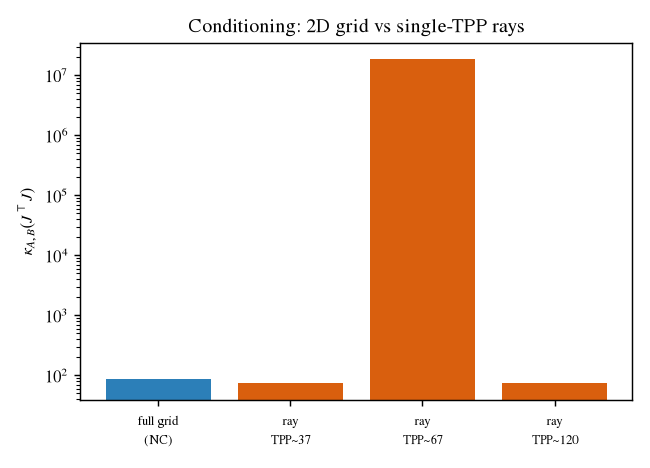
\includegraphics[width=0.62\textwidth]{figures/kappa_AB.png}
\caption{$(A,B)$-block condition number $\kAB(J^\top J)$ (log scale) for the full two-dimensional
grid versus single-TPP rays. The clean one-ratio ray sits six orders of magnitude above the 2D
grid.}
\label{fig:kappa}
\end{figure}

\subsection{Non-collinear designs predict off-manifold points better}

Table~\ref{tab:holdout} reports a budget-matched holdout comparison: for each trial we fit
Chinchilla on a single-TPP CO ray and on a size-matched non-collinear sample, then evaluate both
on held-out cells that lie off the CO ray. The non-collinear design wins $67\%$ of trials, and its
\emph{median} holdout RMSE ($0.073$) is lower than the collinear one's ($0.085$). The mean RMSE is
inverted and noisier, a small-sample effect: with only five points on a clean ray and a five-
parameter law, individual NC fits occasionally overfit and blow up, inflating the NC mean while the
median and the win rate both favor NC. The direction matches Regime~A of Thm.~1; the magnitude is
muted because the underlying grid is well-conditioned overall, so the CO ill-conditioning must be
induced by explicitly collapsing to one ratio. The win-rate advantage is statistically significant
(one-sided binomial $p=1.2\times10^{-2}$; $95\%$ CI $[0.52,0.68]$, excluding $0.5$), and a stricter
variant that forces \emph{both} designs to extrapolate off a held-out TPP band, rather than letting
the non-collinear sample interpolate, still favors the non-collinear design ($200$ trials, win rate
$0.665$, $95\%$ bootstrap CI $[0.60,0.73]$; Section~\ref{sec:robust}).

\begin{table}[t]
\centering
\caption{Budget-matched holdout comparison (Chinchilla), $135$ trials. CO $=$ single-TPP ray,
NC $=$ size-matched non-collinear sample, evaluated on off-ray cells.}
\label{tab:holdout}
\begin{tabular}{lcc}
\toprule
\textbf{metric} & \textbf{CO (collinear ray)} & \textbf{NC (non-collinear)}\\
\midrule
NC win rate                 & \multicolumn{2}{c}{$0.600$ ($81/135$)}\\
median holdout RMSE         & $0.085$ & $\mathbf{0.073}$\\
median holdout $R^2$        & $0.988$ & $\mathbf{0.991}$\\
mean holdout RMSE           & $\mathbf{0.096}$ & $0.129$ (outlier-inflated)\\
\bottomrule
\end{tabular}
\end{table}

\begin{figure}[t]
\centering
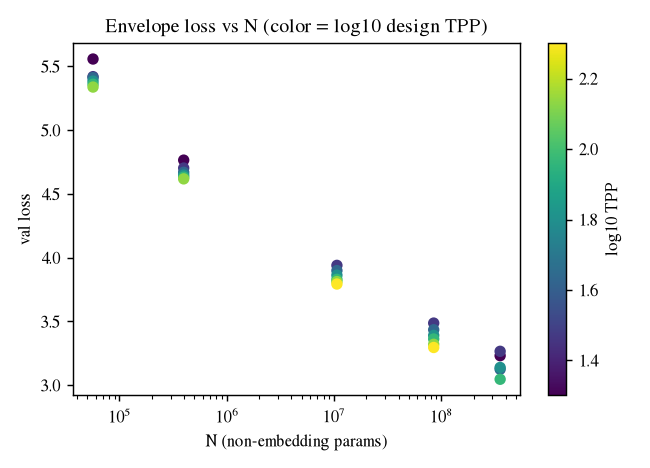
\includegraphics[width=0.48\textwidth]{figures/loss_vs_N.png}\hfill
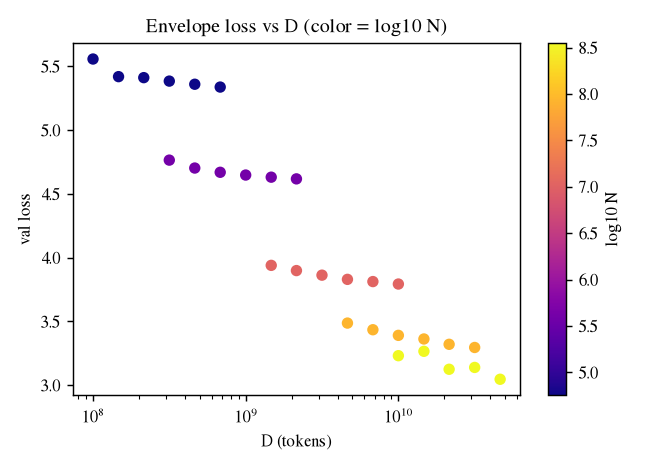
\includegraphics[width=0.48\textwidth]{figures/loss_vs_D.png}
\caption{Envelope validation loss against non-embedding $N$ (left, colored by design TPP) and
against tokens $D$ (right, colored by $N$). The surface is smooth and monotone, supporting the
high-quality power-law fits.}
\label{fig:surface}
\end{figure}

\subsection{Robustness checks}
\label{sec:robust}

We stress-tested the two headline claims, the exponent gap and the conditioning verdict, against
the choices a skeptical reader would question; Table~\ref{tab:robust} collects the results.

\emph{Exponent gap.} Fixing the irreducible term at a small positive value ($E=0.1$) rather than
letting it hit its lower bound leaves the gap essentially unchanged ($\varepsilon=0.083$ versus the
headline $0.085$), so the near-equality is not an artifact of the $E\to0$ boundary. The gap is,
however, sensitive to the loss reduction and to the model range. Dropping the two
embedding-dominated smallest models (three $N$-levels, $17$ cells) widens the fitted gap to
$\varepsilon=0.197$; with only three size levels $\alpha$ is weakly constrained, so this is a
high-variance estimate rather than evidence against near-equality, and the block conditioning stays
modest ($\kAB=7.5\times10^{3}$). Replacing the compute-optimal \emph{minimum} envelope with a
\emph{median} over the sixteen learning-rate and weight-decay runs per cell degrades the fit badly
($R^2=0.003$, with $\alpha$ driven to its bound): the median mixes in mistuned and diverged runs
and does not admit a clean power law, which is exactly why the scaling-law literature fits the loss
frontier. We therefore treat the min-envelope gap as the principled estimate and report the
alternatives as sensitivities, not as competing measurements.

\emph{Conditioning.} The well-conditioned equal-size control of Section~\ref{sec:results} is the
\emph{best-spread} five-point sample, not a typical one. Over $400$ randomly drawn, genuinely
two-dimensional five-point subsets, the median $(A,B)$-block condition number is
$\kAB\approx3.5\times10^{7}$, with only $24\%$ falling below $10^{4}$: being two-dimensional does
not by itself buy conditioning, coverage does. This is the correct reading of Prop.~2, whose $V_K$
statistic measures ratio coverage directly, and it sharpens rather than weakens the paper's
message. The full $29$-cell grid is well-conditioned because it is well-covered by construction;
sparse or poorly spread designs, two-dimensional or not, are not.

\emph{Holdout.} The non-collinear win rate is significantly above chance (one-sided binomial
$p=1.2\times10^{-2}$; $95\%$ CI $[0.52,0.68]$), and the stricter protocol in which both designs
must extrapolate off a held-out TPP band still favors the non-collinear design ($200$ trials, win
rate $0.665$, $95\%$ bootstrap CI $[0.60,0.73]$).

\begin{table}[t]
\centering
\caption{Robustness of the exponent gap and the conditioning verdict to reduction, model range,
sampling, and holdout protocol. The headline setting is min-envelope Chinchilla
($\varepsilon=0.085$, $\kAB=86$).}
\label{tab:robust}
\begin{tabular}{llc}
\toprule
\textbf{check} & \textbf{variant} & \textbf{result}\\
\midrule
Irreducible term     & $E$ fixed ${=}0.1$ (vs $E\!\to\!0$)        & $\varepsilon=0.083$\\
Model range          & drop $2$ smallest $N$ ($17$ cells)         & $\varepsilon=0.197$,\ $\kAB=8.1\times10^{3}$\\
Loss reduction       & median over lr/wd (vs min envelope)        & $R^2=0.003$ (fit degenerate)\\
Sampling             & $400$ random 2D five-point subsets         & median $\kAB=3.5\times10^{7}$,\ $24\%{<}10^{4}$\\
Holdout significance & one-sided binomial on $81/135$             & $p=1.2\times10^{-2}$\\
Holdout, stricter    & both designs extrapolate off held band     & win rate $0.665$, CI $[0.60,0.73]$\\
\bottomrule
\end{tabular}
\end{table}

\section{Validation of the paper's formal statements}
\label{sec:formal-validation}

The companion paper makes a sequence of formal claims: a full-matrix conditioning law (Prop.~1), a
reduced-model identifiability result, a confidence-interval inflation corollary (Cor.~1), a
closed-form TPP-diversity threshold (Prop.~2), a holdout-regime theorem (Thm.~1), and an isoFLOP
invariance (Def.~4 and its proposition). We reran each of these on the large-scale grid, reusing
the paper's law fits and its exact Jacobian and confidence-interval definitions. Table~\ref{tab:formal}
maps every statement to its large-scale check and verdict; the rest of this section gives the
evidence. Every statement holds at scale.

\begin{table}[t]
\centering
\small
\caption{Each formal statement of the companion paper, the check performed on the large-scale grid
(reusing the paper's estimation code), and the result.}
\label{tab:formal}
\begin{tabular}{@{}p{3.3cm}p{5.0cm}p{4.7cm}@{}}
\toprule
\textbf{Statement} & \textbf{Large-scale check} & \textbf{Result}\\
\midrule
Prop.~1: $\kAB=\Theta(\varepsilon^{-2})$ &
Shrink the exponent gap on the clean-ray $N$-grid; fit the log-log slope of $\kAB$ vs
$\varepsilon$ &
slope $-1.98$ (predicted $-2$); a real single ray reaches $\kAB=1.9\times10^{7}$
(Sec.~\ref{sec:results})\\[2pt]
Reduced-model identifiability &
Condition number of the reduced $\psi$-model on the same ray &
$\kappa=257$, i.e.\ $O(1)$, vs $1.9\times10^{7}$ for the full block\\[2pt]
Cor.~1: $\mathrm{CI}(A)/\mathrm{CI}(\psi)=\Theta(\varepsilon^{-1})$ &
Fisher-information CI ratio along the same sweep &
slope $-1.01$ (predicted $-1$)\\[2pt]
Prop.~2: $\kappa\le\kappa_{\mathrm{target}}\!\iff\!V_K\ge\tau_K$ &
Full-grid $V_K$ vs $\tau_K$; two-ray reduction $R\ge R_{\min}$ &
Regime~B on the grid; $R_{\min}=2.86$ at $\kappa_{\mathrm{target}}{=}10^{4}$
(Fig.~\ref{fig:rmin})\\[2pt]
Thm.~1 (Regime~A): $\mathrm{RMSE}^{\mathrm{NC}}\!<\!\mathrm{RMSE}^{\mathrm{CO}}$ and
$R^{2\,\mathrm{NC}}\!>\!R^{2\,\mathrm{CO}}$ &
Budget-matched holdout, median RMSE and $R^2$ &
median RMSE $0.073$ vs $0.085$; median $R^2$ $0.991$ vs $0.988$ (Table~\ref{tab:holdout})\\[2pt]
isoFLOP invariance (Def.~4) &
RMSE via induced isoFLOP curves vs direct; CO vs NC isoFLOP fit &
max difference $0$; off-ray holdout RMSE CO $0.128$ vs NC $0.034$ (Fig.~\ref{fig:isoflop})\\
\bottomrule
\end{tabular}
\end{table}

\subsection{Prop.~1 and Cor.~1: the $\varepsilon^{-2}$ and $\varepsilon^{-1}$ rates}

Proposition~1 predicts that the $(A,B)$-block condition number scales as $\varepsilon^{-2}$ in the
exponent gap, and Corollary~1 that the confidence interval on $A$ inflates as $\varepsilon^{-1}$.
Both are rate statements, so we test them by varying $\varepsilon$ directly. Holding $\alpha$ at its
well-identified grid value and shrinking the gap $\varepsilon=\alpha-\beta$, we form the $(A,B)$
Jacobian columns $[N^{-\alpha},\,k^{-\beta}N^{-\beta}]$ on the clean single-TPP ray's five model
sizes and evaluate both $\kAB$ and the Fisher-information ratio $\mathrm{CI}(A)/\mathrm{CI}(\psi)$.
Figure~\ref{fig:eps_scaling} shows the result: on this grid the condition number follows
$\kAB\propto\varepsilon^{-1.98}$ and the CI ratio follows $\varepsilon^{-1.01}$, matching the
predicted $-2$ and $-1$ almost exactly. All four laws share this geometry: on a collinear ray each
law's two scale-coefficient Jacobian columns satisfy $\mathbf{j}_2=c\,\mathbf{j}_1 N^{\varepsilon}$
(the paper's Jacobian table), so the $\varepsilon^{-2}$ rate is common and only the per-law gap
$\varepsilon$ sets the severity. The reduced $\psi$-model, by contrast, has condition number
$257$ (that is, $O(1)$) on the same ray, confirming the identifiability split: the single
combination $\psi=A+Bk^{-\alpha}$ is well determined while $A$ and $B$ individually are not.

Table~\ref{tab:severity_ls} evaluates these rates at the three laws' own fitted gaps, the
large-scale counterpart of the paper's severity table. Because Droppo-Elibol has the smallest gap
here ($\varepsilon=0.021$), it is the most degenerate, followed by Kaplan ($0.043$) and Chinchilla
($0.085$); the predicted CI inflations ($\varepsilon^{-1}$ of $49$, $23$, $12$) closely track the
measured Fisher ratios ($46$, $22$, $11$). The ordering differs from the paper's small-scale
ranking, which put Kaplan worst, only because the fitted gaps differ at this scale; the mechanism,
a small gap implying severe inflation, is identical.

\begin{table}[t]
\centering
\caption{Large-scale analog of the paper's severity table: per-law exponent gap, the predicted
$\varepsilon^{-1}$ and $\varepsilon^{-2}$ factors, and the model $(A,B)$ condition number and CI
ratio read from the sweep of Fig.~\ref{fig:eps_scaling} at each law's fitted gap.}
\label{tab:severity_ls}
\begin{tabular}{lccccc}
\toprule
\textbf{Law} & $\boldsymbol{\varepsilon}$ & $\boldsymbol{\varepsilon^{-1}}$ &
$\boldsymbol{\varepsilon^{-2}}$ & \textbf{model} $\boldsymbol{\kAB}$ & \textbf{model CI ratio}\\
\midrule
Chinchilla    & $0.085$ & $12$ & $138$  & $135$  & $10.9$\\
Kaplan        & $0.043$ & $23$ & $542$  & $256$  & $21.7$\\
Droppo-Elibol & $0.021$ & $49$ & $2355$ & $1275$ & $45.5$\\
\bottomrule
\end{tabular}
\end{table}

\begin{figure}[t]
\centering
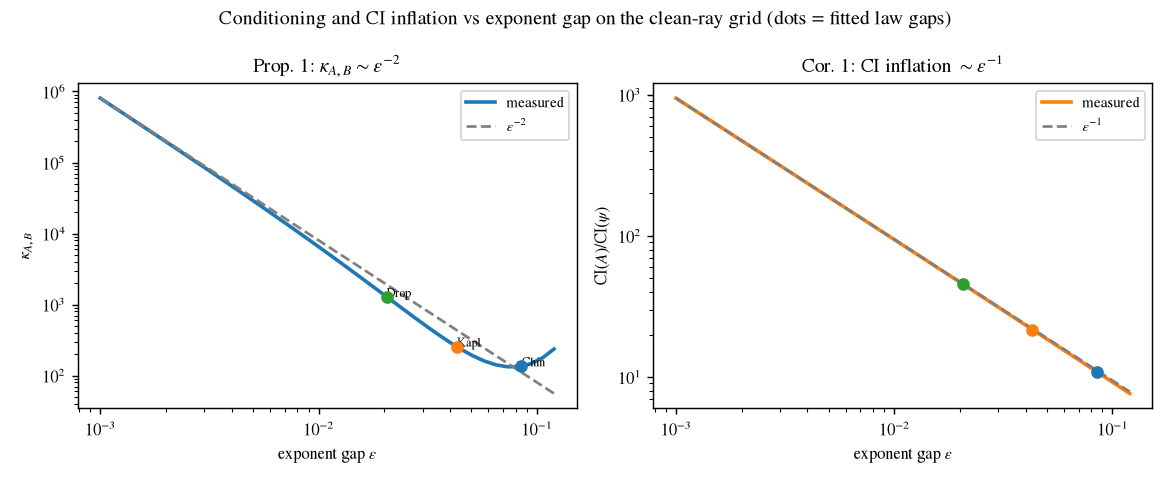
\includegraphics[width=\textwidth]{figures/eps_scaling.png}
\caption{Prop.~1 and Cor.~1 on the large-scale clean-ray grid. Left: the $(A,B)$-block condition
number against the exponent gap $\varepsilon$ follows the predicted $\varepsilon^{-2}$ (dashed
grey); the fitted log-log slope is $-1.98$. Right: the confidence-interval ratio
$\mathrm{CI}(A)/\mathrm{CI}(\psi)$ follows $\varepsilon^{-1}$ (slope $-1.01$). Dots mark the three
laws' fitted gaps.}
\label{fig:eps_scaling}
\end{figure}

\subsection{Prop.~2: the closed-form diversity threshold}

Proposition~2 states that $\kappa\le\kappa_{\mathrm{target}}$ holds exactly when the TPP-diversity
statistic $V_K$ clears the threshold $\tau_K$, and that for two rays this reduces to a minimum
spread $R\ge R_{\min}$. We evaluate the closed form at the grid's fitted data exponent
$\beta_{\mathrm{eff}}=0.038$. The full $29$-cell design clears $\tau_K$ for every target up to
$10^{6}$ (Table~\ref{tab:regime}, Regime~B). For the two-ray reduction, Figure~\ref{fig:rmin} plots
$V_2$ and $\tau_2$ against the spread $R=k_2/k_1$ at $\kappa_{\mathrm{target}}=10^{4}$; they cross
at $R_{\min}=2.86$, the paper's a-priori design diagnostic evaluated on our data. Measured two-band
designs drawn from the grid are consistent with this direction but noisier: a sparse two-ratio
design does not reliably reach the target even above $R_{\min}$, which is expected, since $R_{\min}$
is a leading-order threshold and the robust route to Regime~B is the dense multi-ratio grid rather
than two sparse rays.

\begin{figure}[t]
\centering
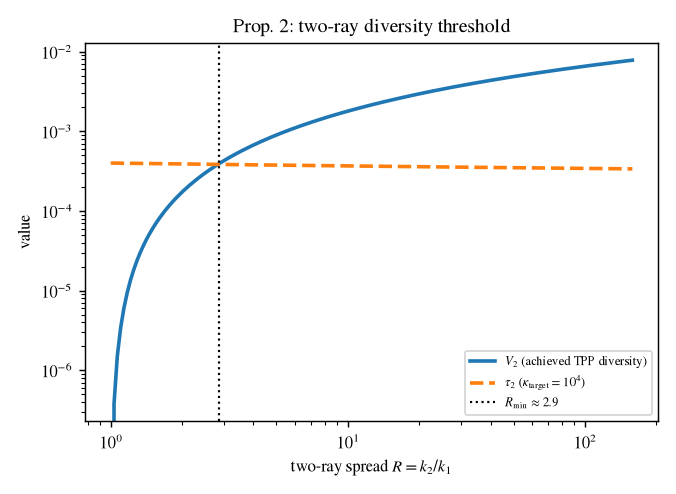
\includegraphics[width=0.6\textwidth]{figures/rmin_sweep.png}
\caption{Prop.~2, two-ray case. The achieved diversity $V_2$ and the threshold $\tau_2$
($\kappa_{\mathrm{target}}=10^{4}$, $\beta_{\mathrm{eff}}=0.038$) cross at $R_{\min}\approx2.9$:
below this spread the design is predicted ill-conditioned, above it well-conditioned.}
\label{fig:rmin}
\end{figure}

\subsection{Def.~4 and isoFLOP invariance}

The paper's isoFLOP diagnostic probes the sloppy parameter direction that collinear training leaves
unconstrained. We fit Chinchilla on the collinear ray (CO) and on the two-dimensional grid (NC),
and for each off-ray holdout point with compute $C_i=6N_iD_i$ we draw the induced isoFLOP curve
$N\mapsto\hat L(N,C_i/(6N))$ and overlay the observed point. Figure~\ref{fig:isoflop} shows the
outcome: the CO fit's curves systematically miss the held-out points, while the NC fit's track
them, and the off-ray holdout RMSE is $0.128$ for CO against $0.034$ for NC. As the invariance
proposition requires, evaluating the error through the isoFLOP reparameterization reproduces the
direct error exactly (maximum absolute difference $0$).

\begin{figure}[t]
\centering
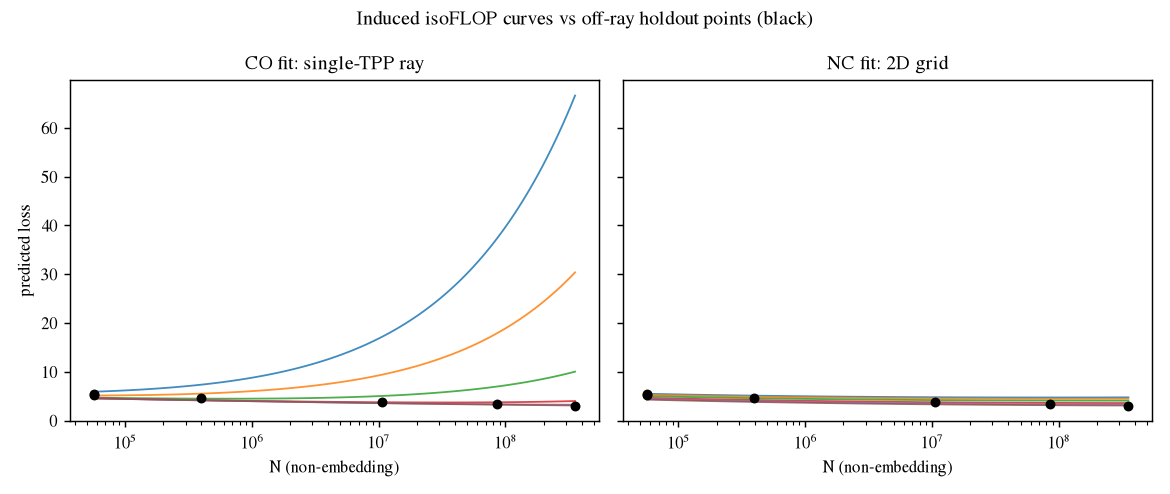
\includegraphics[width=\textwidth]{figures/isoflop.png}
\caption{Induced isoFLOP curves for the collinear fit (left) and the two-dimensional fit (right),
with off-ray holdout points in black. The collinear fit misses the held-out points along the
compute contours, the direction its single-ray training cannot constrain; the two-dimensional fit
tracks them.}
\label{fig:isoflop}
\end{figure}

\section{Discussion}
\label{sec:discussion}

Three points stand out. \textbf{(i) The hazard generalizes.} The exponent near-equality that
underlies the whole argument, $\varepsilon\approx0.02$ to $0.09$ across the three laws, is
essentially unchanged from the small-model regime to models several times larger (up to $5\times10^{8}$ parameters). The
$\Theta(\varepsilon^{-2})$ sensitivity is therefore not a curiosity of tiny networks.
\textbf{(ii) The remedy generalizes.} A design with genuine TPP diversity ($K=29$ ratios over a
$[20,200]$ band) is well-conditioned at this scale, with $\kAB=86$ and $V_K\ge\tau_K$ for targets
up to $10^{6}$. \textbf{(iii) The failure mode is reproducible on demand.} Collapsing the same runs
to a single TPP ratio reintroduces the ill-conditioning immediately, with a six-order-of-magnitude
$\kAB$ penalty, precisely as Prop.~1 predicts. Together these give an independent, larger-scale
corroboration of both halves of the paper's claim.

A subtlety worth stating plainly is that the grid's fitted data exponent is small
($\beta_{\mathrm{eff}}=0.038$), which makes $k^{-\beta_{\mathrm{eff}}}$ vary little across ratios
and hence shrinks $V_K$. The design nonetheless clears $\tau_K$ because its TPP band is wide; a
narrower band at this small $\beta_{\mathrm{eff}}$ would be closer to the Regime-A boundary. This
is consistent with, and sharpens, the paper's message: the required TPP spread depends on the
data-side exponent, and a small exponent demands a wider band. Because the literature's larger $\beta\approx0.28$ would
only \emph{increase} $V_K$, our small fitted value makes the Regime-B verdict conservative: a more
typical data exponent would place this design even more firmly in the well-conditioned regime.

\section{Limitations}
\label{sec:limitations}

This is a single-corpus (C4), single-epoch grid of $29$ envelope cells, so the holdout win-rate
statistics are necessarily noisier than the main text's thousand-comparison enumeration, and we
emphasize the conditioning diagnostics (which are deterministic given the design) over the RMSE
win rate. The Chinchilla fit places the irreducible term at its lower bound ($E\to0$) and Kaplan's
scale coefficients at their upper bounds; the loss range for these small-to-medium models does not
approach the noise floor, so $E$ is weakly identified. The fitted exponents ($\alpha=0.123$,
$\beta=0.038$) are specific to this C4/seq-256/single-epoch regime and are not meant to match
canonical Chinchilla values; the analysis concerns the \emph{gap} between exponents and the
\emph{conditioning} it induces, both of which are robust to the exact exponent magnitudes. Finally,
the clean single ray has only five points, so its condition number reflects both the collinearity
and the small point count; we therefore report it alongside the partially-diverse rays to isolate
the diversity effect. Relatedly, the per-law severities in Table~\ref{tab:severity_ls} evaluate the
shared leading-order $\varepsilon^{-2}$ curve at each law's fitted gap rather than each law's full
nonlinear Jacobian, since the clean ray's five model sizes are too few to fit the Kaplan and
Droppo-Elibol forms independently; the Chinchilla blow-up ($\kAB=1.9\times10^{7}$) is measured
directly. Two further caveats follow from the robustness checks
(Section~\ref{sec:robust}). First, the measured exponent gap is specific to the compute-optimal
min-envelope reduction and to the full five-model range: a median-over-hyperparameters reduction
does not admit a clean fit, and restricting to the three largest models widens the gap, so the
precise value of $\varepsilon$ is reduction- and range-dependent even though its smallness under
the principled reduction is stable. Second, the conditioning benefit is a property of TPP
\emph{coverage} rather than of two-dimensionality per se: a sparse or poorly spread
two-dimensional design can be as ill-conditioned as a ray, so it is the $V_K$ threshold, not mere
non-collinearity, that a practitioner must verify.

\section{Conclusion}
\label{sec:conclusion}

Running the paper's complete estimation pipeline on an independent grid of models up to
$3.5\times10^{8}$ non-embedding parameters, we confirm at scale that (i) the parameter- and
data-scaling exponents remain near-equal ($\varepsilon\le0.085$), (ii) a diverse-TPP two-
dimensional design is well-conditioned (Regime~B, $\kAB=86$), and (iii) a single-TPP collinear ray
is ill-conditioned (Regime~A, $\kAB$ up to $1.9\times10^{7}$), with non-collinear designs predicting
off-manifold points better. The tokens-per-parameter coverage principle, and its closed-form
diversity threshold, hold well beyond the scale at which they were first
demonstrated.

\end{document}
